\documentclass[a4,center,fleqn]{NAR}

% Enter dates of publication
\copyrightyear{2008}
\pubdate{31 July 2009}
\pubyear{2009}
\jvolume{37}
\jissue{12}

\bibliography{paper-webserver.bib}

%\articlesubtype{This is the article type (optional)}

\begin{document}

\title{Article title}

\author{%
Corresponding Author\,$^{1,*}$,
First Co-Author\,$^{2}$
and Second Co-Author\,$^2$%
\footnote{To whom correspondence should be addressed.
Tel: +44 000 0000000; Fax: +44 000 0000000; Email: xxx@yyyy.ac.zz}}

\address{%
$^{1}$Affiliation of Corresponding Author
and
$^{2}$Affiliation of Both Co-Authors}
% Affiliation must include:
% Department name, institution name, full road and district address,
% state, Zip or postal code, country

\history{%
Received January 1, 2009;
Revised February 1, 2009;
Accepted March 1, 2009}

\maketitle

\begin{abstract}
Text. Text. Text. Text. Text. Text. Text. Text. Text. Text. Text.
Text. Text. Text. Text. Text. Text. Text. Text. Text. Text. Text.
Text. Text. Text. Text. Text. Text. Text. Text. Text. Text. Text.
Text. Text. Text. Text. Text. Text. Text. Text. Text. Text. Text.
Text. Text. Text. Text. Text. Text. Text. Text. Text. Text. Text.
Text. Text. Text. Text. Text. Text. Text. Text. Text. Text. Text.
Text. Text. Text. Text. Text. Text. Text. Text. Text. Text. Text.
Text. Text. Text. Text. Text. Text. Text. Text. Text. Text. Text.
Text. Text. Text. Text. Text. Text. Text. Text. Text. Text. Text.
Text. Text. Text. Text. Text. Text. Text. Text. Text. Text. Text.
Text. Text. Text. Text. Text. Text. Text. Text. Text. Text. Text.
Text. Text. Text. Text. Text. Text. Text. Text. Text. Text. Text.
Text. Text. Text. Text. Text. Text. Text. Text. Text. Text. Text.
Text. Text. Text. Text. Text. Text. Text. Text. Text. Text. Text.
Text. Text. Text. Text. Text. Text. Text. Text. Text. Text. Text.
Text. Text. Text. Text. Text. Text. Text. Text. Text. Text. Text.
Text. Text. Text. Text. Text. Text. Text. Text. Text. Text. Text.
Text. Text. Text. Text. Text. Text. Text. Text. Text. Text. Text.
Text. Text. Text. Text. Text. Text. Text. Text. Text. Text. Text.
Text. Text. Text. Text. Text. Text. Text. Text. Text. Text. Text.
Text. Text. Text. Text. Text. Text. Text. Text. Text. Text. Text.
Text. Text. Text. Text. Text. Text. Text. Text. Text. Text. Text.
Text. Text. Text. Text. Text. Text. Text. Text. Text. Text. Text.
Text. Text.
\end{abstract}


\section{Introduction}
Broad --> narrow
-Bacterial infections are a cause of human disease -> associated costs
-Surveillance is used to monitor known pathogens and detect emerging threats, to lower burden of human illness
-Until recently, surveillance involved traditional reference laboratory techniques (and still does) --> examples of both old and new (WGS), what they measure, how they are used
-WGS methods have great potential, but some drawbacks (list with references)
-Some of the drawbacks can be solved by providing pre-computed analyses for routine tasks
-We have previously created SuperPhy, which helps solve some of the issues
-Some issues still remain
-In this study, we have addressed these issues by ... which will provide these benefits

% costs of bacterial infections
Foodborne ilnesses are increasingly difficult to track; ingrediants are globally sourced and contamination can occur at any point in the supply-chain.
The resulting consumer infections translate into actual costs: in Canada, an estimated 4000 hospitalizations and 105 deaths per year are thought to be the result of various pathogens \cite{thomas2015estimates}.
In the United States, 55961 hospitalizations and 1351 deaths per year \cite{scallan2011foodborne} are due to foodborne illnesses.
Futhermore, the associated economic costs have been known for decades \cite{todd1989costs}.
% surveillance
Public-health agencies routinely monitor emerging threats, of which \textit{Salmonella enterica} and \textit{Escherichia coli} are amongst the two most common \cite{kozak2013foodborne}.
In \textit{Salmonella enterica} \cite{bell2016recent}, \textit{Escherichia coli} \cite{fratamico2016advances}, and others pathogens \cite{ronholm2016navigating}, a variety of bioinformatic approaches to surveillance are now based on whole-genome sequencing (WGS).

% traditional reference lab techniques
To begin analyzing genomes, researchers designate particular strains of bacterial isolates using identifiers known as subtypes.
Traditional reference laboratory techniques handled subtyping through methods such as serotyping, pulsed-field gel electrophoresis (PFGE), or Sanger sequencing, amongst others \cite{ronholm2016navigating}.
PFGE is unique amongst the set; restriction enzymes are used to produce DNA fragments visible as specific banding patterns.
Public health agencies use PFGE to track outbreaks by comparing band patterns of isolates \cite{kozak2013foodborne}.
However, as WGS rarely produces complete circular genomes and, in PFGE, cutting by a restriction enzyme is dependent on protein structure, bioinformatic-analogs to PFGE are difficult to develop.
Unlike PFGE, both serotyping and MLST have WGS-based computational methods which mimick results of the wet-lab techniques.
Serotyping uses antibodies to detect the presence of specific cell surface antigens and multi-locus sequence typing (MLST), using Sanger sequencing, examines differences in housekeeping genes which are required to maintain cell function.
By comparing a pre-collected set of reference gene sequences against a WGS result, we can predict wet-lab serotyping results \cite{whiteside2016superphy}, Virulence Factor (VF) results \cite{joensen2014real}, and antimicrobial resistance (AMR) results \cite{mcarthur2013comprehensive}.
A similar approach can be taken for MLST \cite{larsen2012multilocus}.

% potential of WGS
WGS also expands on traditional methods: due to the inclusion of the entire genome, WGS-based methods offer better resolution and context for evaluating the spread of outbreaks \cite{ronholm2016navigating}.
In laboratory-based MLST, instead of examining selected single-nucleotide polymorphisms (SNPs) in a subset of housekeeping genes, newer WGS-based methods, such as core genome MLST (cgMLST), attempt to cover every common gene.
WGS approaches also expands on VF and AMR gene detection to cover every known sequence.
Furthermore, using WGS we can study the relations between genomes, changes in which VF or AMR genes are present over time, and mutations in genes \cite{ronholm2016navigating}.
Entire datasets and results can also be shared in real-time \cite{ronholm2016navigating}.

% Drawbacks - genetics
However, these WGS-based methods only examine the underlying genetics, not the expressed phenotype; the presence of a particular gene sequence does not necessitate expression.
Correspondingly, more target sequences are identified using WGS; if we take a tradition approach to making threat assessments by looking for known VFs or AMR genes, the large number of results make it difficult to guage risk \cite{ronholm2016navigating}.
The effectiveness of WGS-based methods also rely on the accuracy and breadth of reference datasets and agencies must weigh the cost of developing expertise in bioinformatic approaches, while laboratory based phenotypic tests remain inexpensive \cite{koser2012routine}.

% drawbacks - big data
Traditionaly, bioinformatics software was developed \textit{ad hoc} without employing software engineering principles \cite{de2015trends}.
Tools were often script-based, with custom data formats, and only suitable for small collections of data \cite{de2015trends}.
Since WGS-technology expanded the availability of data, systems engineering principles are important to handle code failures across the entire bioinformatics pipeline \cite{schatz2015biological}.
The field also lags behind other big-data industries: bioinformatics software still struggles to perform computations in real-time, stores data in inflexible databases \cite{de2015trends}, and lacks a common application programming interface (API) linking resources \cite{swaminathan2016review}.

% Solution via software engineering
Efforts such as the Comprehensive Antibiotic Resistance Database (CARD) \cite{mcarthur2013comprehensive} attempt to alleviate data concerns by curating a set of known AMR genes.
In addition, agencies such as the Food and Drug Administration (FDA), which hosts GenomeTrakr \cite{allard2016practical}, the National Center for Biotechnology Information (NCBI), which hosts GenBank \cite{doi:10.1093/nar/gks1195}, and the Center for Disease Control and Prevention (CDC), which hosts PulseNet \cite{swaminathan2001pulsenet}, provide services to share genome sequences and associated metadata either openly or amongst member institutions.
Recent efforts have focused on checking the quality of shared reference genomes \cite{parks2015checkm}, particularly amongst human-genome projects \cite{lee2017ngscheckmate}.

% rewrite of bigdata approach (BIGGER bigdata)
While efforts such as CARD as important for replicating traditional results and for historical context, WGS can also be used to develop new methods using the larger datasets available.
To study entire genomes, we need methods of creating reference sets encompassing all genes in a given phlogeny.
Panseq \cite{laing2010pan}, Roary \cite{page2015roary}, chewBBACA \url{https://github.com/mickaelsilva/chewBBACA}, and Graphtyper \cite{Eggertsson148403} are freely available to compute these pan-genomic regions.
Such software approaches must scale to larger datasets than those found in wet-lab approaches.
Also, for uptake by front-line clinicians and laboratories, WGS solutions should perform faster; for example, AMR gene prediction should take less than the typical 18-24 hours required in a reference laboratory \cite{koser2012routine}.
Storing results in a tiered structure, with rapid access available for retrieval while maintaining long-term data storage \cite{schatz2015biological}, would enable developers to address the current interactivity limitations \cite{de2015trends} of bioinformatics software.

% why Superphy
To make bioinformatic approaches user-friendly for front-line clinicians and laboratories, a variety of web services have been developed in Denmark \cite{joensen2014real,larsen2012multilocus}, Taiwan \cite{liu2016construction}, and in collaborations \cite{hasman2015detection}.
While useful, arguably \cite{fricke2014bacterial}, the lack of bioinformatic standards and common infrastructure technologies make it difficult to fully leverage the big-data results from WGS.
Existing software also lack ways to integrate results from multiple genomes, and examine the connections between them.

% Superphy
Previously we developed Superphy \cite{whiteside2016superphy}, an online platform targeting \textit{E. coli} which determines Shiga toxin subtypes, AMR genes using CARD, and provides statistical significance tests between subgroups in associated metadata and pan-genome regions.
However, we struggled to provide real-time computing of results and to accomdate an ever-growing reference database.
Furthermore, due to the various dependencies involved, the platform was difficult for other researchers to independently replicate.

% this study
Here we present Spfy, a complete rewrite of Superphy.
Spfy is backed by a graph database which our analysis modules rely on.
Graph databases focus on describing the relationships between different data, and is one of the emerging \cite{de2015trends} database types being used for biological data.
Spfy takes a modular approach to tool integration and distributes analyses over task queues, thereby allowing modules to run in parallel and address code failures.
Serotyping, VF, AMR predictions are computed within minutes, and results are efficiently stored within the graph.
Furthermore, large-scale analyses, such as epidemiological associations between specific genotypes, biomarkers, host, source, and other metadata, and statistically significance testing of genome markers for user-defined groups, are provided in real-time.
We also containerize services using Docker, a modern approach found in many web servers and proposed to mitigate the complexities of bioinformatic pipelines \cite{di2015impact}.
Docker integration ensures that software dependencies, which typically must be manually installed \cite{doi:10.1093/bioinformatics/btu153,laing2010pan,inouye2014srst2}, are handled automatically.
These changes enable us to provide real-time genome analysis and database storage of results for upwards of 5000 genomes.
All services are publicly available at \url{https://lfz.corefacility.ca/superphy/spfy/}.

\section{MATERIALS AND METHODS}
We designed Spfy's front-end following the Material Design standards \url{https://material.io/}, released by Google.
The user interface is implemented with the React JavaScript library \url{https://facebook.github.io/react/}, by Facebook, as a single-page application to allow efficient data-flow without reloading the website.
Everything is compartmentalized within separate Docker containers where the front-end is networked, through Docker-Compose, to the back-end webserver.

Spfy enables processing of thousands of genome sequences using multiple modules.
By using task queue workers, enabled by the Python-based Redis Queue library \url{https://github.com/nvie/rq}, performance can quickly scale to available infrastructure.
As a bioinformatics tool, we ensured reliability of the platform by integrating the open-source Sentry toolkit \url{https://github.com/getsentry/sentry} for real-time exception tracking.
Containers are orchestrated through Docker-Compose allowing the entire platform: webservers, databases, and task workers, to be easily replicated by other researchers.
We present Spfy as an integrated predictive genomics toolkit for pathogens / \textit{E. coli} which leverages advances in web application development and deployment.

Text. Text. Text. Text. Text. Text. Text. Text. Text. Text. Text.
Text. Text. Text. Text. Text. Text. Text. Text. Text. Text. Text.
Text. Text. Text. Text. Text. Text. Text. Text. Text. Text. Text.
Text. Text. Text. Text. Text. Text. Text. Text. Text. Text. Text.
Text. Text. Text. Text. Text. Text. Text. Text. Text. Text. Text.
Text. Text. Text. Text. Text. Text. Text. Text. Text. Text. Text.
Text. Text. Text. Text. Text. Text. Text. Text. Text. Text. Text.
Text. Text. Text{}. Text.
Text \cite{1}.

Text. Text. Text. Text. Text. Text. Text. Text. Text. Text. Text.
Text. Text. Text. Text. Text. Text. Text. Text. Text. Text. Text.
Text. Text. Text. Text. Text. Text. Text. Text. Text. Text. Text.
Text. Text. Text. Text. Text. Text. Text. Text. Text. Text. Text.
Text. Text. Text. Text. Text. Text. Text. Text. Text. Text. Text.
Text. Text. Text. Text. Text. Text. Text. Text. Text. Text. Text.
Text. Text. Text. Text. Text. Text. Text. Text. Text. Text. Text.
Text. Text. Text. Text. Text. Text. Text. Text. Text. Text. Text.
Text. Text. Text. Text. Text. Text. Text. Text. Text. Text. Text.
\begin{align*}
&\mathrm{Ascorbate} + \mathrm{EDTA} \cdot \mathrm{Fe}^{3+} \to
\hbox{Oxidized ascorbate}
\\
&\mathrm{EDTA} \cdot \mathrm{Fe}^{2+} + \mathrm{H}_2
\mathrm{O}_2 \to
\mathrm{EDTA} \cdot \mathrm{Fe}^{3+} + \cdot
\mathrm{OH} + \mathrm{OH}^-
\end{align*}
Text. Text. Text. Text. Text. Text. Text. Text. Text. Text. Text.
Text. Text. Text. Text. Text. Text. Text. Text. Text. Text. Text.
Text. Text. Text. Text. Text. Text. Text. Text. Text. Text. Text.
Text. Text. Text. Text. Text. Text. Text. Text. Text. Text. Text.

Text. Text. Text. Text. Text. Text. Text. Text. Text. Text. Text.
Text. Text. Text. Text. Text. Text. Text. Text. Text. Text. Text.
Text. Text. Text. Text. Text. Text. Text. Text. Text. Text. Text.
Text. Text. Text. Text. Text. Text. Text. Text. Text. Text. Text.
Text. Text. Text. Text. Text. Text. Text. Text. Text. Text. Text.
Text. Text. Text. Text. Text. Text. Text. Text. Text. Text. Text.
Text. Text. Text. Text. Text. Text. Text. Text. Text. Text. Text.
Text. Text. Text. Text. Text. Text. Text. Text. Text. Text. Text.
Text. Text. Text. Text. Text. Text. Text. Text. Text. Text. Text.
Text. Text. Text. Text. Text. Text. Text. Text. Text. Text. Text.
Text. Text. Text. Text. Text. Text. Text. Text. Text. Text. Text.
Text. Text. Text. Text. Text. Text. Text. Text. Text. Text. Text.
% **************************************************************
% Keep this command to avoid text of first page running into the
% first page footnotes
\enlargethispage{-65.1pt}
% **************************************************************

Text. Text. Text. Text. Text. Text.
Text. Text. Text. Text. Text. Text. Text. Text. Text. Text. Text.
Text. Text. Text. Text. Text. Text. Text. Text. Text. Text. Text.
Text. Text. Text. Text. Text. Text. Text. Text. Text. Text. Text.
Text. Text. Text. Text. Text. Text. Text. Text. Text. Text. Text.
Text. Text. Text. Text. Text. Text. Text. Text. Text. Text. Text.
Text. Text. Text. Text. Text. Text. Text. Text. Text. Text. Text.
Text. Text. Text. Text. Text. Text. Text. Text. Text. Text. Text.
Text. Text. Text. Text. Text. Text. Text. Text. Text. Text. Text.
Text. Text. Text. Text. Text. Text. Text. Text. Text. Text. Text.
Text. Text. Text. Text. Text. Text. Text. Text. Text. Text. Text.
Text. Text. Text. Text. Text. Text. Text. Text. Text. Text. Text.
Text. Text. Text. Text. Text. Text. Text. Text. Text. Text. Text.
Text. Text. Text. Text. Text. Text. Text. Text. Text. Text. Text.
Text. Text. Text. Text. Text. Text. Text. Text. Text. Text. Text.
Text. Text. Text. Text. Text. Text. Text. Text. Text. Text. Text.
Text. Text. Text. Text.
Text \cite{2,3}.

Text. Text. Text. Text. Text. Text. Text. Text. Text. Text. Text.
Text. Text. Text. Text. Text. Text. Text. Text. Text. Text. Text.
Text. Text. Text. Text. Text. Text. Text. Text. Text. Text. Text.
Text. Text. Text. Text. Text. Text. Text. Text. Text. Text. Text.
Text. Text. Text. Text. Text. Text. Text. Text. Text. Text. Text.
Text. Text. Text. Text. Text. Text. Text. Text. Text. Text. Text.
Text. Text. Text. Text. Text. Text. Text. Text. Text. Text. Text.
Text. Text. Text. Text. Text. Text. Text. Text. Text. Text. Text.
Text. Text. Text. Text. Text. Text. Text. Text. Text. Text. Text.
Text. Text.

Text. Text. Text. Text. Text. Text. Text. Text. Text. Text. Text.
Text. Text. Text. Text. Text. Text. Text. Text. Text. Text. Text.
Text. Text. Text. Text. Text. Text. Text. Text. Text. Text. Text.
Text. Text. Text. Text. Text. Text. Text. Text. Text. Text. Text.
Text. Text. Text. Text. Text. Text. Text. Text. Text. Text. Text.
Text. Text. Text. Text. Text. Text. Text. Text. Text. Text. Text.
Text. Text. Text. Text. Text. Text. Text. Text. Text. Text. Text.
Text. Text. Text. Text. Text. Text. Text. Text. Text. Text. Text.
Text. Text. Text. Text. Text. Text. Text. Text. Text. Text. Text.
Text. Text. Text. Text. Text. Text. Text. Text. Text. Text. Text.
Text. Text. Text. Text. Text. Text. Text. Text. Text. Text. Text.
Text. Text. Text. Text. Text. Text. Text. Text. Text. Text. Text.
Text. Text. Text. Text. Text. Text. Text. Text. Text. Text. Text.
Text. Text. Text. Text. Text. Text. Text. Text. Text. Text. Text.
Text. Text. Text. Text. Text. Text. Text. Text. Text. Text. Text.
Text. Text. Text. Text. Text. Text. Text. Text.
Text \cite{4}.


\section{MATERIALS AND METHODS}

\subsection{Materials subsection one}

Text. Text. Text. Text. Text. Text. Text. Text. Text. Text. Text.
Text. Text. Text. Text. Text. Text. Text. Text. Text. Text. Text.
Text. Text. Text. Text. Text. Text. Text. Text. Text. Text. Text.
Text. Text. Text. Text. Text. Text. Text. Text. Text. Text. Text.
Text. Text. Text. Text. Text. Text. Text. Text. Text. Text. Text.
Text. Text. Text. Text. Text. Text. Text. Text. Text. Text. Text.
Text. Text. Text. Text. Text. Text. Text. Text. Text. Text. Text.
Text. Text. Text. Text. Text. Text. Text. Text. Text. Text. Text.
Text. Text. Text. Text. Text. Text. Text. Text. Text. Text. Text.
Text. Text. Text. Text. Text. Text. Text. Text. Text. Text. Text.
Text. Text. Text. Text. Text. Text. Text. Text. Text. Text. Text.
Text. Text. Text. Text. Text. Text. Text. Text. Text. Text. Text.
Text. Text. Text. Text. Text. Text. Text. Text. Text. Text. Text.
Text. Text. Text. Text. Text. Text. Text. Text. Text. Text. Text.
Text. Text. Text. Text. Text. Text. Text. Text. Text. Text. Text.
Text. Text. Text. Text. Text. Text. Text. Text. Text. Text. Text.
Text. Text. Text. Text. Text. Text. Text. Text. Text. Text. Text.
Text. Text. Text. Text. Text. Text. Text. Text. Text. Text. Text.
Text. Text. Text. Text. Text. Text. Text. Text. Text. Text. Text.
Text. Text. Text. Text. Text. Text. Text. Text. Text. Text. Text.
Text. Text. Text. Text. Text. Text. Text. Text. Text. Text. Text.
Text. Text. Text. Text. Text. Text. Text. Text. Text. Text. Text.
Text. Text. Text. Text. Text. Text. Text. Text. Text. Text. Text.
Text. Text. Text. Text. Text. Text. Text. Text. Text. Text.


\subsubsection{Materials subsubsection one.}

Text. Text. Text. Text. Text. Text. Text. Text. Text. Text. Text.
Text. Text. Text. Text. Text. Text. Text. Text. Text. Text. Text.
Text. Text. Text. Text:
\begin{align}
\mathrm{LD}^r = \frac{\mathrm{LD}}{A_\mathrm{iso}}
= 1.5 S \left( 3 \cos^2 \alpha_i - 1 \right)
\end{align}
Text. Text. Text. Text. Text. Text. Text. Text. Text. Text. Text.
Text. Text. Text. Text. Text. Text. Text. Text. Text. Text. Text.
Text. Text. Text. Text. Text. Text. Text. Text. Text. Text. Text.
Text. Text. Text. Text. Text. Text. Text. Text. Text. Text. Text.
Text. Text. Text. Text. Text. Text. Text. Text. Text. Text. Text.
Text. Text. Text. Text. Text. Text. Text. Text. Text. Text. Text.
Text. Text. Text. Text. Text. Text. Text. Text. Text. Text. Text.
Text. Text. Text. Text. Text. Text. Text. Text. Text. Text. Text.
Text. Text. Text. Text. Text. Text. Text. Text. Text. Text. Text.
Text. Text. Text. Text. Text. Text. Text. Text. Text. Text. Text.
Text. Text. Text. Text. Text. Text. Text. Text. Text. Text. Text.
Text. Text. Text. Text. Text. Text. Text. Text. Text. Text. Text.


\subsection{Materials subsection two}

Text. Text. Text. Text. Text. Text. Text. Text. Text. Text. Text.
Text. Text. Text. Text. Text. Text. Text. Text. Text. Text. Text.
Text. Text. Text. Text. Text. Text. Text
(see Figure \ref{NAR-fig1}).

Text. Text. Text. Text. Text. Text. Text. Text. Text. Text. Text.
Text. Text. Text. Text. Text. Text. Text. Text. Text. Text. Text.
Text. Text. Text. Text. Text. Text. Text. Text. Text. Text. Text.
Text. Text. Text. Text. Text. Text. Text. Text. Text. Text. Text.
Text. Text. Text. Text. Text. Text. Text.
\begin{equation*}
\mathrm{LD} \left( t \right) =
\sum\limits_i
a_i \exp \left( \frac{-t}{\tau_i} \right)
\end{equation*}
Text. Text. Text. Text. Text. Text. Text. Text. Text. Text. Text.
Text. Text. Text. Text. Text. Text. Text. Text. Text. Text. Text.
Text. Text. Text. Text. Text. Text. Text. Text. Text. Text. Text.
Text. Text. Text. Text. Text. Text. Text. Text. Text. Text. Text.
Text. Text. Text. Text. Text. Text. Text. Text. Text. Text. Text.
Text. Text. Text. Text. Text. Text. Text. Text. Text. Text. Text.
Text. Text. Text. Text.

\begin{figure}[t]
\begin{center}
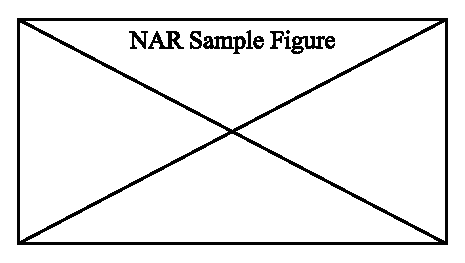
\includegraphics{NAR-fig1.eps}
\end{center}
\caption{Caption for figure within column.}
\label{NAR-fig1}
\end{figure}


\section{RESULTS}

\subsection{Results subsection one}

Text. Text. Text. Text. Text. Text. Text. Text. Text. Text. Text.
Text. Text. Text. Text. Text. Text. Text. Text. Text. Text. Text.
Text. Text. Text. Text. Text. Text. Text. Text. Text. Text. Text.
Text. Text. Text. Text. Text. Text. Text. Text. Text. Text. Text.
Text. Text. Text. Text. Text. Text. Text. Text. Text. Text. Text.
Text. Text. Text. Text. Text. Text. Text. Text. Text. Text. Text.
Text. Text. Text. Text. Text. Text. Text. Text. Text. Text. Text.
Text. Text. Text. Text. Text. Text. Text. Text. Text. Text. Text.
Text. Text. Text. Text. Text. Text. Text. Text. Text. Text. Text.
Text. Text. Text. Text. Text. Text. Text. Text. Text. Text. Text.
Text. Text. Text. Text. Text. Text. Text. Text. Text. Text. Text.
Text. Text. Text. Text. Text. Text. Text. Text. Text.

\begin{table}[b]
\tableparts{%
\caption{This is a table caption}
\label{table:01}%
}{%
\begin{tabular*}{\columnwidth}{@{}lllll@{}}
\toprule
Col. head 1 & Col. head 2 & Col. head 3 & Col. head 4 & Col. head 5
\\
& (\%) & (s$^{-1}$) & (\%) & (s$^{-1}$)
\\
\colrule
Row 1 & Row 1 & Row 1 & -- & --
\\
Row 2 & Row 2 & Row 2 & Row 2 & Row 2
\\
\botrule
\end{tabular*}%
}
{This is a table footnote}
\end{table}


\subsection{Results subsection two}

Text.  Text. Text. Text. Text. Text. Text. Text. Text. Text. Text.
Text. Text. Text. Text. Text. Text. Text. Text. Text. Text. Text.
Text (see Table \ref{table:01}).

Text. Text. Text. Text. Text. Text.
Text. Text. Text. Text. Text. Text. Text. Text. Text. Text. Text.
Text. Text. Text. Text. Text. Text. Text. Text. Text.
Text (see Figure \ref{NAR-fig2}a).

Text. Text. Text. Text. Text.
Text. Text. Text. Text. Text. Text. Text. Text. Text. Text. Text.
Text. Text. Text. Text. Text. Text. Text. Text. Text. Text. Text.
Text. Text. Text. Text. Text. Text. Text. Text. Text. Text. Text.
Text. Text. Text. Text. Text. Text. Text. Text. Text. Text. Text.
Text. Text. Text. Text. Text. Text. Text. Text. Text. Text. Text.
Text. Text. Text. Text. Text. Text. Text. Text. Text. Text. Text.
Text. Text. Text. Text. Text. Text. Text. Text. Text. Text. Text.
Text. Text. Text. Text. Text. Text. Text. Text. Text. Text. Text.
Text. Text. Text. Text. Text. Text. Text. Text. Text. Text. Text.
Text. Text. Text. Text. Text. Text. Text. Text. Text. Text. Text.
Text. Text. Text. Text. Text. Text. Text. Text. Text. Text.

\begin{figure*}[t]
\begin{center}
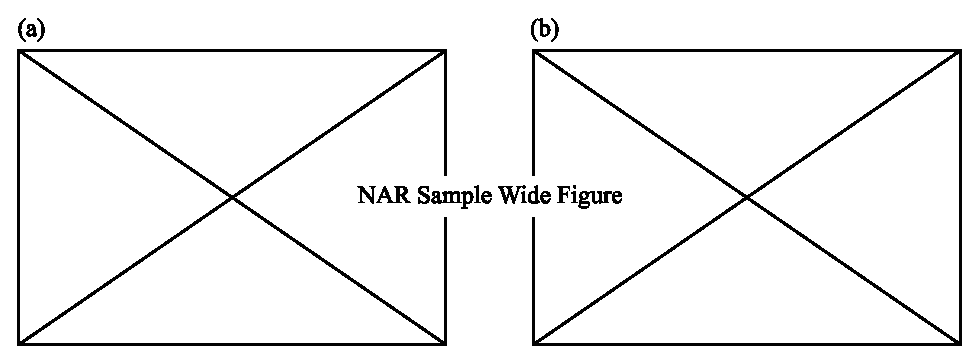
\includegraphics{NAR-fig2.eps}
\end{center}
\caption{Caption for wide figure over two columns.
\textbf{(a)} Left figure.
\textbf{(b)} Right figure (see (a)).
}
\label{NAR-fig2}
\end{figure*}


\subsection{Results subsection three}

Text. Text. Text. Text. Text. Text. Text. Text. Text. Text. Text.
Text. Text. Text. Text. Text. Text. Text. Text. Text. Text. Text.
Text. Text. Text. Text. Text. Text. Text. Text. Text. Text. Text.
Text. Text. Text. Text. Text. Text. Text. Text. Text. Text. Text.
Text. Text. Text. Text. Text. Text. Text. Text. Text. Text. Text.
Text. Text. Text. Text. Text. Text. Text. Text. Text. Text. Text.
Text. Text. Text. Text. Text. Text. Text. Text. Text. Text. Text.
Text. Text. Text. Text. Text. Text. Text. Text. Text. Text. Text.
Text. Text. Text. Text. Text. Text. Text. Text. Text. Text. Text.
Text. Text. Text. Text. Text. Text. Text. Text. Text. Text. Text.
Text. Text. Text.


\section{DISCUSSION}

\subsection{Discussion subsection one}

Text. Text. Text. Text. Text. Text. Text. Text. Text. Text. Text.
Text. Text. Text. Text. Text. Text. Text. Text. Text. Text. Text.
Text. Text. Text. Text. Text. Text. Text. Text. Text. Text. Text.
Text. Text. Text. Text. Text. Text. Text. Text. Text. Text. Text.
Text. Text. Text. Text. Text. Text. Text. Text. Text. Text. Text.
Text. Text. Text. Text. Text. Text. Text. Text. Text. Text. Text.
Text. Text. Text. Text. Text. Text. Text. Text. Text. Text. Text.
Text. Text. Text. Text. Text. Text. Text. Text. Text. Text. Text.
Text. Text. Text. Text. Text. Text. Text. Text. Text. Text. Text.
Text. Text. Text. Text. Text. Text. Text. Text. Text. Text. Text.
Text. Text. Text. Text. Text. Text. Text. Text. Text. Text. Text.
Text. Text. Text. Text. Text. Text. Text. Text. Text. Text. Text.
Text. Text. Text. Text. Text. Text. Text. Text. Text. Text. Text.
Text. Text. Text. Text. Text. Text. Text. Text. Text. Text. Text.
Text. Text. Text. Text. Text. Text. Text. Text. Text. Text. Text.
Text. Text. Text. Text. Text. Text. Text. Text. Text. Text. Text.
Text. Text. Text. Text. Text. Text. Text. Text. Text. Text. Text.
Text. Text. Text. Text. Text. Text. Text. Text. Text. Text. Text.
Text. Text. Text. Text. Text. Text. Text. Text. Text. Text. Text.
Text. Text. Text. Text. Text. Text. Text. Text. Text. Text. Text.
Text. Text. Text. Text. Text. Text.


\subsection{Discussion subsection two}

Text. Text. Text. Text. Text. Text. Text. Text. Text. Text. Text.
Text. Text. Text. Text. Text. Text. Text. Text. Text. Text. Text.
Text. Text. Text. Text. Text. Text. Text. Text. Text. Text. Text.
Text. Text. Text. Text. Text. Text. Text. Text. Text. Text. Text.
Text. Text. Text. Text. Text. Text. Text. Text. Text. Text. Text.
Text. Text. Text. Text. Text. Text. Text. Text. Text. Text. Text.
Text. Text. Text. Text. Text. Text. Text. Text. Text. Text. Text.
Text. Text. Text. Text. Text. Text. Text. Text. Text. Text. Text.
Text. Text. Text. Text. Text. Text. Text. Text. Text. Text. Text.
Text. Text. Text. Text. Text. Text. Text. Text. Text. Text. Text.
Text.

Text. Text. Text. Text. Text. Text. Text. Text. Text. Text. Text.
Text. Text. Text. Text. Text. Text. Text. Text. Text. Text. Text.
Text. Text. Text. Text. Text. Text. Text. Text. Text. Text. Text.
Text. Text. Text. Text. Text. Text. Text. Text. Text. Text. Text.
Text. Text. Text. Text. Text. Text. Text. Text. Text. Text. Text.
Text. Text. Text. Text. Text. Text. Text. Text. Text. Text. Text.
Text. Text. Text. Text. Text. Text. Text. Text. Text. Text. Text.
Text. Text. Text. Text. Text. Text. Text. Text. Text. Text. Text.
Text. Text. Text. Text. Text. Text. Text. Text. Text. Text. Text.
Text. Text. Text. Text. Text. Text. Text. Text. Text. Text. Text.
Text. Text. Text. Text. Text. Text. Text. Text. Text. Text.


\subsection{Discussion subsection three}

Text. Text. Text. Text. Text. Text. Text. Text. Text. Text. Text.
Text. Text. Text. Text. Text. Text. Text. Text. Text. Text. Text.
Text. Text. Text. Text. Text. Text. Text. Text. Text. Text. Text.
Text. Text. Text. Text. Text. Text. Text. Text. Text. Text. Text.
Text. Text. Text. Text. Text. Text. Text. Text. Text. Text. Text.
Text. Text. Text. Text. Text. Text. Text. Text. Text. Text. Text.
Text. Text. Text. Text. Text. Text. Text. Text. Text. Text. Text.
Text. Text. Text. Text. Text. Text. Text. Text. Text. Text. Text.
Text. Text. Text. Text. Text. Text. Text. Text. Text. Text. Text.
Text. Text. Text. Text. Text. Text. Text. Text. Text. Text. Text.
Text. Text. Text. Text. Text. Text. Text. Text. Text.

Text. Text. Text. Text. Text. Text. Text. Text. Text. Text. Text.
Text. Text. Text. Text. Text. Text. Text. Text. Text. Text. Text.
Text. Text. Text. Text. Text. Text. Text. Text. Text. Text. Text.
Text. Text. Text. Text. Text. Text. Text. Text. Text. Text. Text.
Text. Text. Text. Text. Text. Text. Text. Text. Text. Text. Text.
Text. Text. Text. Text. Text. Text. Text. Text. Text. Text. Text.
Text. Text. Text. Text. Text. Text. Text. Text. Text. Text. Text.
Text. Text. Text. Text. Text. Text. Text.

Text. Text. Text. Text. Text. Text. Text. Text. Text. Text. Text.
Text. Text. Text. Text. Text. Text. Text. Text. Text. Text. Text.
Text. Text. Text. Text. Text. Text. Text. Text. Text. Text. Text.
Text. Text. Text. Text. Text. Text. Text. Text. Text. Text. Text.
Text. Text. Text. Text. Text. Text. Text. Text. Text. Text. Text.
Text. Text. Text. Text. Text. Text. Text. Text. Text. Text. Text.
Text. Text. Text. Text. Text. Text. Text. Text. Text. Text. Text.
Text. Text. Text. Text. Text. Text. Text.


\section{CONCLUSION}

Text. Text. Text. Text. Text. Text. Text. Text. Text. Text. Text.
Text. Text. Text. Text. Text. Text. Text. Text. Text. Text. Text.
Text. Text. Text. Text. Text. Text. Text. Text. Text. Text. Text.
Text. Text. Text. Text. Text. Text. Text. Text. Text. Text. Text.
Text. Text. Text. Text. Text. Text. Text. Text. Text. Text. Text.
Text. Text. Text. Text. Text. Text. Text. Text. Text. Text. Text.
Text. Text. Text. Text. Text. Text. Text. Text. Text. Text. Text.
Text. Text. Text. Text. Text. Text. Text. Text. Text. Text. Text.
Text. Text. Text. Text. Text. Text. Text. Text. Text. Text. Text.
Text. Text. Text.


\section{ACKNOWLEDGEMENTS}

Text. Text. Text. Text. Text. Text. Text. Text. Text. Text. Text.
Text. Text. Text. Text.


\subsubsection{Conflict of interest statement.} None declared.
\newpage


\begin{thebibliography}{4}

% Format for article
\bibitem{1}
Author,A.B. and Author,C. (1992)
Article title.
\textit{Abbreviated Journal Name}, \textbf{5}, 300--330.

% Format for book
\bibitem{2}
Author,D., Author,E.F. and Author,G. (1995)
\textit{Book Title}.
Publisher Name, Publisher Address.

% Format for chapter in book
\bibitem{3}
Author,H. and Author,I. (2005)
Chapter title.
In
Editor,A. and Editor,B. (eds),
\textit{Book Title},
Publisher Name, Publisher Address,
pp.\ 60--80.

% Another article
\bibitem{4}
Author,Y. and Author,Z. (2002)
Article title.
\textit{Abbreviated Journal Name}, \textbf{53}, 500--520.

\end{thebibliography}

\end{document}
